\chapter{Benchmark}
Il primo elaborato consta di un \emph{Linux I/O benchmark} per le operazioni di lettura e scrittura su di un file binario. Le dimensioni di file valutate sono:
\begin{itemize}
	\item $10MB$
	\item $100MB$
	\item $1GB$
\end{itemize}
Le operazioni di I/O avvengono a blocchi di dimensione:
\begin{itemize}
	\item $1KB$
	\item $10KB$
	\item $100KB$
	\item $1MB$
\end{itemize}
Il sistema utilizzato è composto da:
\begin{itemize}
	\item processore \texttt{Intel Celeron N3050} $1.60GHz$
	\item memoria RAM DDR3 $4GB$
	\item disco \texttt{HGST HTS545050A7} $500GB$
\end{itemize}
Sono stati effettuati $30$ esperimenti per ogni configurazione attraverso uno script \emph{bash}. Prima di ogni esperimento sono stati utilizzati i comandi \emph{sync} ed $echo\ 1 > /proc/sys/vm/drop\_caches$ per ottenere l'indipendenza tra essi (purge della cache).\par 
Si è sfruttata la direttiva \texttt{O\_DIRECT} all'apertura dei file, per minimizzare l'effetto della cache nelle operazioni di I/O da e verso il file. Ciò ha richiesto l'utilizzo di blocchi allineati, multipli di 512 byte, la cui creazione è stata demandata alla funzione \emph{posix\_memalign}. Il calcolo del tempo è effettuato con \emph{gettimeofday}, ed è attuato in microsecondi.

	\section{Lettura}
		Per effettuare le operazioni di lettura, si è sfruttato un unico file \emph{prova.bin} di $1GB$, creato in precedenza. Si sfruttano le direttive della primitiva \emph{open} che consentono la lettura del file e la lettura diretta dallo storage.
		\lstinputlisting[]{./codice/benchmarkI.c}
	
	\section{Scrittura}
		Le operazioni di scrittura sono effettuate sul file \emph{test.bin}, che viene creato, se già esistente, o altrimenti sovrascritto. Ciò è definito dalle direttive della primitiva \emph{open}, che inoltre indicano l'apertura in scrittura del file, da attuare direttamente verso lo storage. Nel caso di creazione del file, si indicano anche i permessi che esso dovrà avere. L'operazione utilizza un blocco allineato, inizializzato con numeri psudocasuali.
		\lstinputlisting[]{./codice/benchmarkO.c}
		
	\section{Caratterizzazione dei dati misurati}
		I dati sono stati riuniti in tabelle relative alla stessa dimensione di file ed analizzati tramite \emph{JMP}. Si è studiata la distribuzione degli esperimenti di una stessa configurazione, tramite istogramma, e si è valutato il modo migliore per sintetizzare i dati. In particolare, per distribuzioni poco \emph{skewed}, è stata usata la media, la deviazione standard, e l'intervallo di confidenza della media al $95\%$.
		\begin{figure}[H]
			\centering
			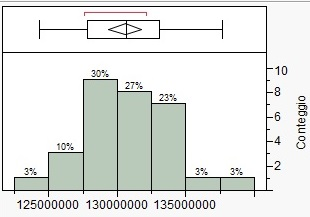
\includegraphics[]{./immagine/W100MBx100KB.jpg}
			\caption{Scrittura di un file di $100MB$ con blocchi di $100KB$}
			\label{fig:b-w100}
		\end{figure}
		In caso di distribuzioni skewed ed eventuali \emph{outlier}, si è optato per la mediana ed il SIQR.
				\begin{figure}[H]
			\centering
			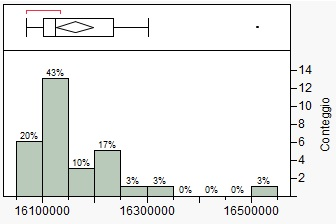
\includegraphics[]{./immagine/R1GBx1MB.jpg}
			\caption{Lettura di un file di $1GB$ con blocchi di $1MB$}
			\label{fig:b-r1}
		\end{figure}
		Sono stati quindi prodotti due data set, contenenti i dati delle operazioni di lettura e scrittura.
		\begin{figure}[H]
			\centering
			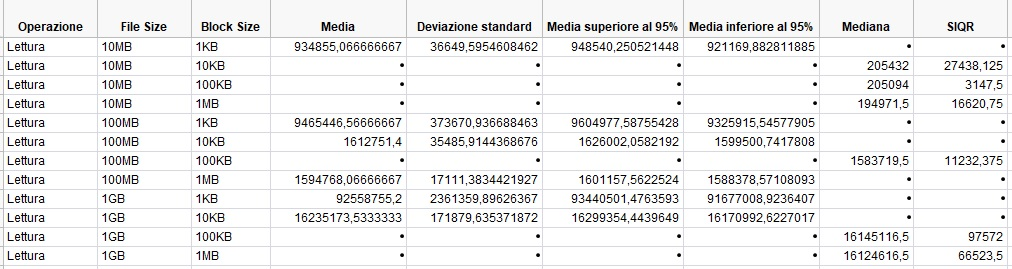
\includegraphics[width=17cm, height= 7cm]{./immagine/letture.jpg}
			\caption{Dati delle letture}
			\label{fig:b-r}
		\end{figure}
		\begin{figure}[H]
			\centering
			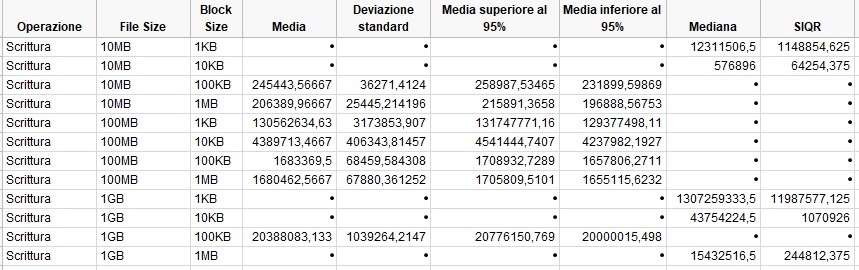
\includegraphics[width=17cm, height=7cm]{./immagine/scritture.jpg}
			\caption{Dati delle scritture}
			\label{fig:b-w}
		\end{figure}
		Si possono, inoltre, sfruttare i risultati ricavati per determinare la dimensione del campione necessaria per ottenere con accuratezza desiderata la media delle osservazioni con un certo livello di confidenza. Prendiamo in considerazione la scrittura di un file di $100MB$. I tempi medi stimati per effettuare l'operazione sono circa: $2.10min$ per blocchi di $1KB$, $4.4s$ per blocchi di $10KB$, $1.7s$ per blocchi di $100KB$, $1.7s$ per blocchi di $1MB$. Si può voler calcolare in questi casi un tempo accurato di $r=0.5\%$ con livello di confidenza del $95\%$. In questi casi, si ricaverebbe una media dei tempi accurata rispettivamente per al più di $6.5ds$, $22ms$, $8.4ms$, $8.4ms$. Si applica dunque:
		\begin{equation}
			n=\left( \frac{100zs}{r\bar{x}}\right) ^{2}
		\end{equation}
		con $z=1.96$, $s$ deviazione standard, $\bar{x}$ media. Si ottiene, quindi, il numero di punti necessari: $n=90$, $n=1316$, $n=254$, $n=250$.
